\subsection*{4.1 SCtickets type}
- introduce details of tickets
\noindent The SCtickets types in AAA are presented in \autoref{fig:type}.
\begin{figure}[h!]
  \centering
  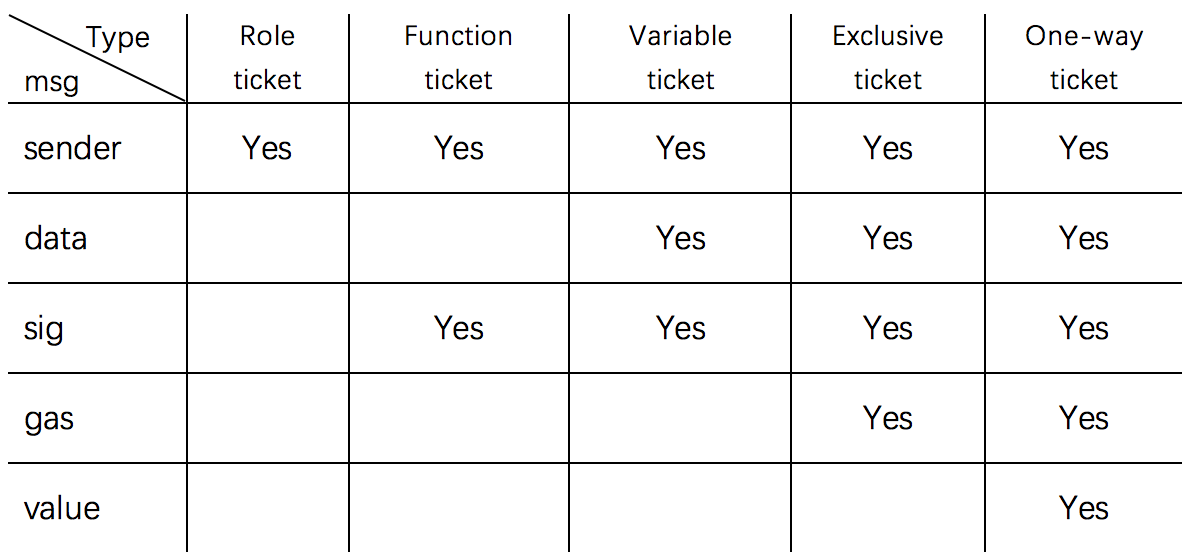
\includegraphics[width=1.0\linewidth]{fig/type}
  \caption{Different SCtickets types granted by AAA.}
  \label{fig:type}
\end{figure}
\\\indent Currently, AAA provides user with five different types of tickets, namely, role tickets, Tx tickets, function \& variable tickets, exclusive tickets and single permit. Different types of tickets should generate different signature which is to be verified by Owner accroding to different neccessary msg information.
\\\textbf{Role ticket}: is the highest priority tickets granted by AAA, meaning that certain caller(a.k.a User) could access to the smart contract before the expiry timestamp freely, regardless of functions, variables, times of sending transactions.
\\\textbf{Function ticket}: provides User with multiple transaction-sending access and full parameters. Hence, it is neccessary for AAA to get the information of msg.sender and msg.sig so as to Owner is aware of which method is to be called in every period of transaction.
\\\textbf{Variable ticket}: limits User to execute specific function code, and besides, variables. AAA parses first four bytes of the full msg.data and following bytes, which represent the function name and input parameters, respectively. Function \& variable ticket can protect some private data member in smart contract from being modified.
\\\textbf{Exclusive ticket}: disallowed other user to access smart contract which is called by current user. By default, other types of tickets are not exclusive by User. Assume that user, who is holding exclusive ticket, is calling the "setter" function of one smart contract. Exclusive ticket gurantees only one user is able to call certain smart contract. Other User will receive deny message from smart contract saying "the tickets is belong to other user now". However, it is not proper that only one user can access to certain contract as time period is too long, e.g., 1 week or 1 month, sometimes. Hence, Exclusive ticket need msg.gas for the fact that blockchain can notice the timestamp when obtaining msg.gas, which means remaining gas and transaction is done. After that, other User is able to access to previous smart contract.
\\\textbf{One-way ticket}: gurantees the User only get access to the smart contract one time though holding a valid SCtickets authorized by AAA system as the name implies. In order to generate one-trip ticket, AAA need to get as much as information to tag transaction well. When double-sending happends, smart contract emits deny User's access infomation if former transaction information has been stored.

\subsection*{4.2 Tickets implementation}
- introduce implementation tickets type 
- introduce each tickets msg data, usage, applicable scenario

\noindent \textbf{1a}): Owner represents the address that a smart contract is initially created. In Ethereum world, every valid account hold its own private key which could be regarded as an unique idendity. Obviously, the owner of a smart contract need to generate a key-pair only for signature and verification when constructing new smart contract and synchronize private key with AAA party. Firstly, Owner uses keccak256(private\_key, nounce) to produce a new private key where private\_key represents its own account pk and nounce only valid for current smart contract. After that, a new key-pair is created by getting the return value of privateKeyToAccount(). We define a localStorage object, namely, keyStorage, to store address-to-privatekey mapping in AAA and this object is essential to Node.js storage package. Meanwhile, keep the public key of above-mentioned key-pair in Owner's smart contract for verified signature.
\\\noindent \textbf{1b}): Policies vary in different smart contracts and could be customized by Owner. Compared with key-related API, Owner is also supposed to update its own policies with AAA. Like key pair, AAA maintains a policy storage area to save all the policies corresponding to certain Owner. Currently,  every single policy struct has two member for test convenience: balance, to rule the access balance limit; time, to set access period. Like 1a), AAA also provides APIs which Owner is able to add, delete, update policies. 
\\\noindent \textbf{2a,2b,2c}): Once completely updated policy and synchronized private key to AAA, Owner is to be called by User all the time. This process starts with applyTickets(type, msg, policy\_info) defined in AAA system. First of all, User calls applyTickets() function with the input argument of type, namely, tickets type, msg, calling data and policy\_info, which contains ample value of User. And then, AAA is responsible for determining if User meets policies defined by Owner by matching every rules in policy structure. If lucky, AAA grants valid ticket to User. A valid ticket contains several data parts: one is tickets type. At present, we tag five types of tickets discussed in Chapter4.1 from integer 1 to 5 representing five types respectively. Signature part contains signed data by Owner private key generated by web3.eth.accounts.sign() in web3.js package and hash of msg for following signature validation process. The value of msg varies according to diffrent tickets type. More importantly, ticket definitely returns timestamp value to Owner so as to synchronize the access peroid between Owner and User.
\\\noindent \textbf{3a}): User sends transaction to the smart contract of Owner after obtaining valid tickets from AAA. In our case, setA() function, defined in Owner smart contract, is to alter value of a, which is an uint type storage in Owner. We assume that User is willing to update a's value by calling Owner.setA() along with ticket dicussed above.
\\\noindent \textbf{3b}): After noticing the calling message from User, Owner implement verified() to gives priority to verify the validation of ticket. Normally, the validation process need to be done two steps. One is vefify the current timestamp \textgreater  access period or not. Second step is done by wrapping parseTickets() function which accepts two parameter, hash of message and signature. Owner needs to parse the signature manually and retrieve three parameters r, s, and v, the first 32 bytes of signature, the 33-64 bytes of signature and the recover arguments for ECC respectively. In ethereum, the value of v is usually set 27. Finally, we get the public key which is corrensponding to the private key signing the message by leverage the ecrecover() in Solidity. If the return valus equals to the address of Owner, which means the ticket verified successfully, User can hold this valid tickets to access to the Owner's smart contract. Furthermore, there needs to be one more step for one-trip ticket. Owner need to look for and determine if the id is in set or not.


\subsection*{4.3 One-way tickets}
- introduce motivation, backgroud, difficulty, scenario
- introduce implementation, bit-map synchronization process

\subsection*{4.4 Tickets among Multiple smart contract}
- introduce tickets transfer among external calling contract
- introduce append tickets and updated tickets verification process



